\begin{figure}[H]
\centering
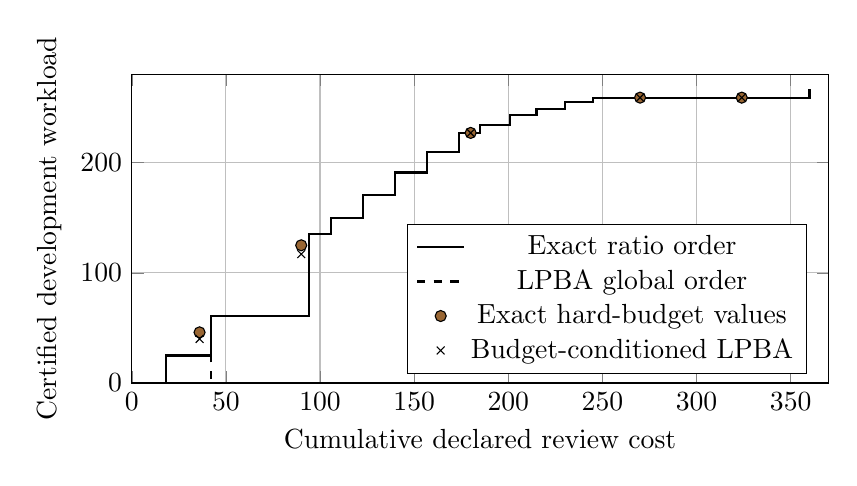
\begin{tikzpicture}
\begin{axis}[width=.86\textwidth,height=5.5cm,xlabel={Cumulative declared review cost},ylabel={Certified development workload},xmin=0,xmax=370,ymin=0,ymax=280,grid=major,legend pos=south east]
\addplot+[black,thick,mark=none,const plot] coordinates {(0.0,0.0) (2.0,0.0) (18.0,25.0) (42.0,61.0) (94.0,135.0) (106.0,150.0) (123.0,171.0) (140.0,191.0) (157.0,210.0) (174.0,227.0) (185.0,234.0) (201.0,243.0) (215.0,249.0) (230.0,255.0) (245.0,259.0) (360.0,267.0)};
\addlegendentry{Exact ratio order}
\addplot+[black,dashed,thick,mark=none,const plot] coordinates {(0.0,0.0) (42.0,61.0) (94.0,135.0) (106.0,150.0) (123.0,171.0) (140.0,191.0) (157.0,210.0) (174.0,227.0) (185.0,234.0) (201.0,243.0) (215.0,249.0) (230.0,255.0) (245.0,259.0) (360.0,267.0)};
\addlegendentry{LPBA global order}
\addplot+[only marks,mark=*,black] coordinates {(36.0,46.0) (90.0,125.0) (180.0,227.0) (270.0,259.0) (324.0,259.0)};
\addlegendentry{Exact hard-budget values}
\addplot+[only marks,mark=x,black] coordinates {(36.0,40.0) (90.0,117.0) (180.0,227.0) (270.0,259.0) (324.0,259.0)};
\addlegendentry{Budget-conditioned LPBA}
\end{axis}
\end{tikzpicture}
\caption{One document-derived banking catalog. Step lines show completed-packet authority in whole-order schedules; isolated markers are separately optimized hard-budget outcomes. The connected lines do not interpolate the fixed-budget optima.\label{fig:bank}}
\end{figure}
